\chapter{Implementation}

\section{Concretizing Arguments}
Concretizing a list of arguments is done iteratively by deep copying the abstract AF $F'$ to create a new AF $F''$ and mutating it. The mutation is guided by five steps considering the unchanged abstract AF $F'$ and the concrete AF $F$. To improve the understanding of each step, we accompany the explanation with the example depicted in \ref{example:concretizationOfArguments}, where we concretize the arguments $a$ and $b$.

\vspace{0.3cm}
\begin{figure}[h]
    \begin{minipage}{.475\textwidth}
        \centering
        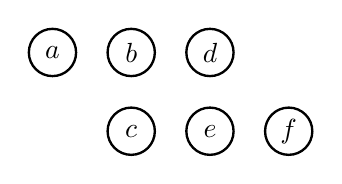
\begin{tikzpicture}
            % Singletons
                \def \ax{0}   \def \ay{0}
                \def \bx{1}   \def \by{0}
                \def \cx{1}   \def \cy{-1}
                \def \dx{2}   \def \dy{0}
                \def \ex{2}   \def \ey{-1}
                \def \fx{3}   \def \fy{-1}

                \draw[line width=0.3mm] (\ax, \ay) circle (0.3) node[anchor=center]{$a$};
                \draw[line width=0.3mm] (\bx, \by) circle (0.3) node[anchor=center]{$b$};
                \draw[line width=0.3mm] (\cx, \cy) circle (0.3) node[anchor=center]{$c$};
                \draw[line width=0.3mm] (\dx, \dy) circle (0.3) node[anchor=center]{$d$};
                \draw[line width=0.3mm] (\ex, \ey) circle (0.3) node[anchor=center]{$e$};
                \draw[line width=0.3mm] (\fx, \fy) circle (0.3) node[anchor=center]{$f$};
                % Attacks
                \DrawAttackHorizontal{L}{\bx}{\by}{\ax}{\ay}
                \DrawAttackHorizontal{L}{\dx}{\dy}{\bx}{\by}

                \DrawAttackVertical{D}{\bx}{\by}{\cx}{\cy}
                \DrawAttackVertical{U}{\ex}{\ey}{\dx}{\dy}

                \DrawAttackDiagonal{NRL}{\cx}{\cy}{\ax}{\ay}
        \end{tikzpicture}
        \captionof{figure}{Concrete AF $F$}
    \end{minipage}%
    \begin{minipage}{.475\textwidth}
        \centering
        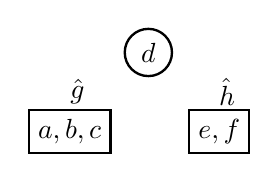
\begin{tikzpicture}
            % Singletons
            \def \dx{1}   \def \dy{0}
            \def \gx{0}   \def \gy{-1}
            \def \hx{1.9}   \def \hy{-1}

            \draw[line width=0.3mm] (\dx, \dy) circle (0.3) node[anchor=center]{$d$};
            % Cluster
        
            \node[rectangle, draw, line width=0.3mm] at (\gx, \gy) {$a,b,c$};
            \node at (\gx + 0.1, \gy+0.5) {$\hat{g}$};

            \node[rectangle, draw, line width=0.3mm] at (\hx, \hy) {$e,f$};
            \node at (\hx + 0.1, \hy+0.5) {$\hat{h}$};

            % Attacks
            \DrawAttackDiagonal{PRL}{\dx}{\dy}{\gx+0.1}{\gy+0.1}
            \DrawAttackDiagonal{NRL}{\hx}{\hy+0.1}{\dx}{\dy}
            \DrawSelfAttackLeftTopCluster{\gx-0.45}{\gy+0.3}

            % \DrawAttackDiagonal{NRL}{\cx}{\cy}{\ax}{\ay}
        \end{tikzpicture}
        \captionof{figure}{Abstract AF $F'$}

    \end{minipage}
    \caption{Example: Concretization of arguments}
    \label{example:concretizationOfArguments}
\end{figure}

\vspace{-0.2cm}

\paragraph{Step 1:} Each argument needing concretization is first removed from the parent cluster and added as a singleton in $F''$. 
If an argument is not part of a cluster or is invalid, we remove it and continue with the filtered valid list.
We do not consider attacks in this step since they depend on the concrete- and abstract AFs.


\vspace{0.3cm}
\begin{figure}[h]
    \centering
    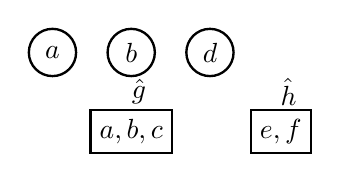
\begin{tikzpicture}
        % Singletons
        \def \ax{0}   \def \ay{0}
        \def \bx{1}   \def \by{0}
        \def \dx{2}   \def \dy{0}
        \def \gx{1}   \def \gy{-1}
        \def \hx{2.9}   \def \hy{-1}

        \draw[line width=0.3mm] (\ax, \ay) circle (0.3) node[anchor=center]{$a$};
        \draw[line width=0.3mm] (\bx, \by) circle (0.3) node[anchor=center]{$b$};
        \draw[line width=0.3mm] (\dx, \dy) circle (0.3) node[anchor=center]{$d$};
        % Cluster

        \node[rectangle, draw, line width=0.3mm] at (\gx, \gy) {$a,b,c$};
        \node at (\gx + 0.1, \gy + 0.5) {$\hat{g}$};

        \node[rectangle, draw, line width=0.3mm] at (\hx, \hy) {$e,f$};
        \node at (\hx + 0.1, \hy + 0.5) {$\hat{h}$};

        % Attacks
        \DrawAttackDiagonal{PRL}{\dx}{\dy}{\gx+0.1}{\gy+0.1}
        \DrawAttackDiagonal{NRL}{\hx}{\hy+0.1}{\dx}{\dy}
        \DrawSelfAttackLeftTopCluster{\gx-0.45}{\gy+0.3}

    \end{tikzpicture}
    \caption{Concretized AF $F''$ after Step 1}
\end{figure}
\vspace{-0.2cm}


\paragraph{Step 2:} We add the new attacks from all concretized arguments to the remaining clusters. We must do this after
removing the arguments from the clusters because if an argument $a$ attacks argument $b$ in the concrete AF, and $b$ is part of the cluster $F'$ in the abstract AF, by concretizing $b$, the attack $(a,F')$ would not be valid anymore.


\vspace{0.3cm}
\begin{figure}[h]
    \centering
    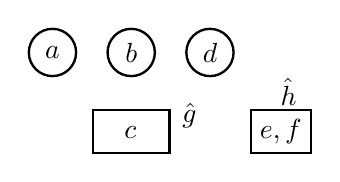
\begin{tikzpicture}
        % Singletons
        \def \ax{0}   \def \ay{0}
        \def \bx{1}   \def \by{0}
        \def \dx{2}   \def \dy{0}
        \def \gx{1}   \def \gy{-1}
        \def \hx{2.9}   \def \hy{-1}

        \draw[line width=0.3mm] (\ax, \ay) circle (0.3) node[anchor=center]{$a$};
        \draw[line width=0.3mm] (\bx, \by) circle (0.3) node[anchor=center]{$b$};
        \draw[line width=0.3mm] (\dx, \dy) circle (0.3) node[anchor=center]{$d$};
        % Cluster

        \node[rectangle, draw, line width=0.3mm] at (\gx, \gy) {$\phantom{a,} c\phantom{, b}$};
        \node at (\gx + 0.74, \gy + 0.2) {$\hat{g}$};

        \node[rectangle, draw, line width=0.3mm] at (\hx, \hy) {$e,f$};
        \node at (\hx + 0.1, \hy + 0.5) {$\hat{h}$};

        % Attacks
        \DrawAttackDiagonal{PRL}{\dx}{\dy}{\gx+0.1}{\gy+0.1}
        \DrawAttackDiagonal{NRL}{\hx}{\hy+0.1}{\dx}{\dy}
        \DrawSelfAttackLeftTopCluster{\gx-0.45}{\gy+0.3}
        \DrawAttackVertical{D}{\bx}{\by}{\gx}{\gy}
        \DrawAttackDiagonal{NRL}{\gx-0.1}{\gy+0.1}{\ax}{\ay}


    \end{tikzpicture}
    \caption{Concretized AF $F''$ after Step 2}
\end{figure}
\vspace{-0.2cm}


\paragraph{Step 3:} After adding the new attacks, we need to check which attacks from $F'$ are still valid in $F''$. If an attack is not valid
anymore through the concretization, we remove it in $F''$. An attack is not valid anymore; if we remove one of the arguments being attacked or attacked by argument $a$ from the cluster $f$ and no other attack exists, s.t. $a$ is attacked from/attacking an argument within $f$. Selfattacks of clusters could also change by the concretization of arguments. Therefore, we need to check the clusters from which the arguments are concretized. 


\vspace{0.3cm}
\begin{figure}[h]
    \centering
    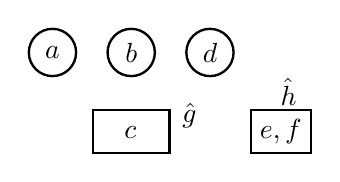
\begin{tikzpicture}
        % Singletons
        \def \ax{0}   \def \ay{0}
        \def \bx{1}   \def \by{0}
        \def \dx{2}   \def \dy{0}
        \def \gx{1}   \def \gy{-1}
        \def \hx{2.9}   \def \hy{-1}

        \draw[line width=0.3mm] (\ax, \ay) circle (0.3) node[anchor=center]{$a$};
        \draw[line width=0.3mm] (\bx, \by) circle (0.3) node[anchor=center]{$b$};
        \draw[line width=0.3mm] (\dx, \dy) circle (0.3) node[anchor=center]{$d$};
        % Cluster

        \node[rectangle, draw, line width=0.3mm] at (\gx, \gy) {$\phantom{a,} c\phantom{, b}$};
        \node at (\gx + 0.74, \gy + 0.2) {$\hat{g}$};

        \node[rectangle, draw, line width=0.3mm] at (\hx, \hy) {$e,f$};
        \node at (\hx + 0.1, \hy + 0.5) {$\hat{h}$};

        % Attacks
        \DrawAttackDiagonal{NRL}{\hx}{\hy+0.1}{\dx}{\dy}
        \DrawAttackVertical{D}{\bx}{\by}{\gx}{\gy}
        \DrawAttackDiagonal{NRL}{\gx-0.1}{\gy+0.1}{\ax}{\ay}
    \end{tikzpicture}
    \caption{Concretized AF $F''$ after Step 3}
\end{figure}
\vspace{-0.2cm}


\paragraph{Step 4:} In this step we add the new attacks between the singletons. Due to the fact, that we copied all the attacks from $F'$, we only have to take into consideration the attacks from or to the concretized singletons. So instead of iterating over all singletons of the AF, we can limit the attack creation to the concretized singletons. 


\vspace{0.3cm}
\begin{figure}[h]
    \centering
    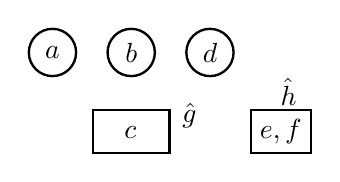
\begin{tikzpicture}
        % Singletons
        \def \ax{0}   \def \ay{0}
        \def \bx{1}   \def \by{0}
        \def \dx{2}   \def \dy{0}
        \def \gx{1}   \def \gy{-1}
        \def \hx{2.9}   \def \hy{-1}

        \draw[line width=0.3mm] (\ax, \ay) circle (0.3) node[anchor=center]{$a$};
        \draw[line width=0.3mm] (\bx, \by) circle (0.3) node[anchor=center]{$b$};
        \draw[line width=0.3mm] (\dx, \dy) circle (0.3) node[anchor=center]{$d$};
        % Cluster

        \node[rectangle, draw, line width=0.3mm] at (\gx, \gy) {$\phantom{a,} c\phantom{, b}$};
        \node at (\gx + 0.74, \gy + 0.2) {$\hat{g}$};

        \node[rectangle, draw, line width=0.3mm] at (\hx, \hy) {$e,f$};
        \node at (\hx + 0.1, \hy + 0.5) {$\hat{h}$};

        % Attacks
        \DrawAttackDiagonal{NRL}{\hx}{\hy+0.1}{\dx}{\dy}
        \DrawAttackVertical{D}{\bx}{\by}{\gx}{\gy}
        \DrawAttackDiagonal{NRL}{\gx-0.1}{\gy+0.1}{\ax}{\ay}
        \DrawAttackHorizontal{L}{\dx}{\dy}{\bx}{\by}
        \DrawAttackHorizontal{L}{\bx}{\by}{\ax}{\ay}
    \end{tikzpicture}
    \caption{Concretized AF $F''$ after Step 4}
\end{figure}
\vspace{-0.2cm}


\paragraph{Step 5:} The last step is to clean up the argumentation framework $F''$ by removing all empty clusters and mutating the clusters with exactly
one singleton to the mentioned singleton. 


\vspace{0.3cm}
\begin{figure}[h!]
    \centering
    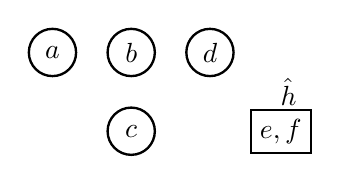
\begin{tikzpicture}
        % Singletons
        \def \ax{0}   \def \ay{0}
        \def \bx{1}   \def \by{0}
        \def \dx{2}   \def \dy{0}
        \def \cx{1}   \def \cy{-1}
        \def \hx{2.9}   \def \hy{-1}

        \draw[line width=0.3mm] (\ax, \ay) circle (0.3) node[anchor=center]{$a$};
        \draw[line width=0.3mm] (\bx, \by) circle (0.3) node[anchor=center]{$b$};
        \draw[line width=0.3mm] (\cx, \cy) circle (0.3) node[anchor=center]{$c$};
        \draw[line width=0.3mm] (\dx, \dy) circle (0.3) node[anchor=center]{$d$};
        % Cluster
        \node[rectangle, draw, line width=0.3mm] at (\hx, \hy) {$e,f$};
        \node at (\hx + 0.1, \hy + 0.5) {$\hat{h}$};

        % Attacks
        \DrawAttackDiagonal{NRL}{\hx}{\hy+0.1}{\dx}{\dy}
        \DrawAttackVertical{D}{\bx}{\by}{\cx}{\cy}
        \DrawAttackDiagonal{NRL}{\cx}{\cy}{\ax}{\ay}
        \DrawAttackHorizontal{L}{\dx}{\dy}{\bx}{\by}
        \DrawAttackHorizontal{L}{\bx}{\by}{\ax}{\ay}
    \end{tikzpicture}
    \caption{Concretized AF $F''$ after Step 5}
\end{figure}
\vspace{-0.2cm}

\restoregeometry
